\section{Timeline of Live Electronic Ensemble}

\subsection{A visualization of the history of live electronic ensemble music with relevant people and events.}

%-----------------------------------------------------------
% Visualization of Timeline Leading to Live Electronic Ensembles

\begin{center}
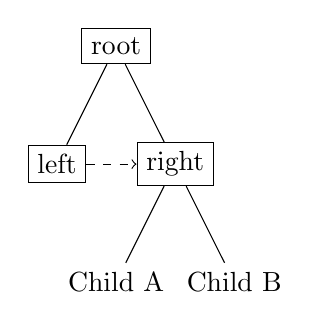
\begin{tikzpicture}[sibling distance=15mm]
    
  \node[rectangle,draw] {root}
    child {node[rectangle,draw] (left node) {left}}
    child {
        node[rectangle,draw] (right node) {right}
            child {node {Child A}}
		child {node {Child B}}
    };
  \draw[dashed,->] (left node) -- (right node);

\end{tikzpicture}
\end{center}

% %-----------------------------------------------------------

% %-----------------------------------------------------------
% % Timeline using TikZ
% % Designs obtained from https://stackoverflow.com/questions/217834/how-to-create-a-timeline-with-latex

% %Basic timeline

% \chronoperiodecoloralternation{orange, green,
% red, yellow, pink}
% \startchronology
% \chronoperiode[startdate=false]{0}{500}{}
% \chronoperiode[startdate=false]{500}{1000}{}
% \chronoperiode[startdate=false]{1000}{1500}{}
% \chronoperiode{1500}{1800}{Anything you want}
% \chronoperiode{1800}{1950}{18\textsuperscript{th} century}
% \chronoperiode{1950}{2100}{Anything you want}
% \stopchronology

% \setupchronology{startyear=1000,color=blue,stopdate=false}
% \setupchronoperiode{color=green}
% \setupchronoevent{textstyle=\it}
% \setupchronograduation[event]{markdepth=2cm}
% \startchronology
% \chronograduation{250}
% \chronoperiode{1050}{1450}{Anything you want}
% \chronoevent{1600}{Anything else}
% \chronoperiode{1800}{1899}{19\textsuperscript{th} century}
% \stopchronology

% \startchronology[startyear=-800,stopyear=500,
% color=green, height=3cm]
% \chronoperiode[color=orange,bottomdepth=1cm, topheight=2cm,
% textstyle=\it, dateselevation=-15pt, ifcolorbox=false,
% box=true]{-753}{-509}{Roman Royal period}
% \chronoperiode[color=cyan,startdate=false, textstyle=\bf,
% textdepth=35pt, bottomdepth=1cm, topheight=2cm,
% ifcolorbox=false, dateselevation=-15pt,
% box=true]{-509}{-27}{Roman Republic}
% \stopchronology

% %Straight Timeline
% \begin{tikzpicture}[remember picture, overlay, shift={(0,-3.5)}]

%   % Starting point at (0,0) on the page
%   \coordinate (start) at (0,0);

%   % Draw the first line: 25 degrees, 9cm length
%   \draw[color = blue!40, line join=round, line cap=round, shading angle=25, opacity=0.5, top color=blue!10, bottom color=blue!60] (start) -- ++(-30:9cm) coordinate (end1); 

%   % Draw the second line: -20 degrees, 9.5cm length
%   \draw[color = blue!40, line join=round, line cap=round, shading angle=-20, opacity=0.5, top color=blue!10, bottom color=blue!60] (start) -- ++(-26:9.5cm) coordinate (end2

%   % Fill the space between the lines with blue and reduced opacity
%   \begin{scope}
%     \path[clip] (start) -- (end1) -- (end2) -- cycle;
%     \shade[bottom color=blue!10, top color=blue!60, opacity=0.5] (start) rectangle (end2|-end1);
%   \end{scope}

%   % Draw ovals at the starting point
%   \draw[color = red, fill = red, opacity = 0.8, line width=0.01cm] (start) ++(-28:0.3cm) ellipse [x radius=0.05cm, y radius=0.012cm];
%   \draw[color = orange, fill = orange, opacity = 0.8, line width=0.01cm] (start) ++(-28:2.2cm) ellipse [x radius);=0.115cm, y radius=0.055cm];
%   \draw[color = yellow, fill = yellow, opacity = 0.8, line width=0.01cm] (start) ++(-28:3.8cm) ellipse [x radius=0.18cm, y radius=0.11cm];
%   \draw[color = green, fill = green, opacity = 0.8, line width=0.01cm] (start) ++(-27.95:6.2cm) ellipse [x radius=0.355cm, y radius=0.15cm];
%   \draw[color = teal, fill = teal, opacity = 0.8, line width=0.01cm] (start) ++(-27.95:8cm) ellipse [x radius=0.42cm, y radius=0.21cm];

%   % Draw ovals around the existing ovals
%   \draw[color = red, line width = 0.005cm] (start) ++(-28:0.3cm) ellipse [x radius=0.05*1.5cm, y radius=0.012cm*1.5];
%   \draw[color = orange, line width = 0.005cm] (start) ++(-28:2.2cm) ellipse [x radius=0.115cm*1.5, y radius=0.055cm*1.5];
%   \draw[color = yellow, line width = 0.005cm] (start) ++(-28:3.8cm) ellipse [x radius=0.18cm*1.5, y radius=0.11cm*1.5];
%   \draw[color = green, line width = 0.005cm] (start) ++(-27.95:6.2cm) ellipse [x radius=0.355cm*1.5, y radius=0.15cm*1.5];
%   \draw[color = teal, line width = 0.005cm] (start) ++(-27.95:8cm) ellipse [x radius=0.42cm*1.3, y radius=0.21cm*1.3];

%   % Draw perpendicular lines going up 3cm
%   \draw[color = red, dashed, opacity=0.8] (start) ++(-28:0.3cm) -- ++(90:3.5cm) node[right, scale = 0.9, color = red] {1997};
%   \draw[color = orange, dashed, opacity=0.8] (start) ++(-28:2.2cm) -- ++(90:3.5cm) node[right, scale=0.9, color = orange] {2004};
%   \draw[color = yellow, dashed, opacity=0.8] (start) ++(-28:3.8cm) -- ++(90:3.5cm) node[right, scale=0.9, color = yellow] {2005};
%   \draw[color = green, dashed, opacity=0.8] (start) ++(-27.95:6.2cm) -- ++(90:3.5cm) node[right, scale=0.9, color = green] {2007};
%   \draw[color = teal, dashed, opacity=0.8] (start) ++(-27.95:8cm) -- ++(90:3.5cm) node[right, scale=0.9, color = teal] {2010};

%   % Add text under the years
%   \node[right, color = black, scale = 0.5] (1) at ($(start) + (-28:0.4cm) + (90:3cm)$) {Lorem};
%   \node[right, color = black, scale = 0.5] (2) at ($(start) + (-28:0.4cm) + (90:2.8cm)$) {ipsum dolor};
%   \node[right, color = black, scale = 0.5] (3) at ($(start) + (-28:2.3cm) + (90:3cm)$) {Lorem};
%   \node[right, color = black, scale = 0.5] (4) at ($(start) + (-28:2.3cm) + (90:2.8cm)$) {ipsum dolor};
%   \node[right, color = black, scale = 0.5] (5) at ($(start) + (-28:3.9cm) + (90:3cm)$) {Lorem ipsum};
%   \node[right, color = black, scale = 0.5] (6) at ($(start) + (-28:3.9cm) + (90:2.8cm)$) {dolor sit};
%   \node[right, color = black, scale = 0.5] (7) at ($(start) + (-28:3.9cm) + (90:2.6cm)$) {amet};
%   \node[right, color = black, scale = 0.5] (8) at ($(start) + (-28:6.3cm) + (90:3cm)$) {Lorem};
%   \node[right, color = black, scale = 0.5] (9) at ($(start) + (-28:6.3cm) + (90:2.8cm)$) {ipsum};
%   \node[right, color = black, scale = 0.5] (10) at ($(start) + (-28:8.1cm) + (90:3cm)$) {Lorem};
%   \node[right, color = black, scale = 0.5] (11) at ($(start) + (-28:8.1cm) + (90:2.8cm)$) {ipsum dolor};
%   \node[right, color = black, scale = 0.5] (12) at ($(start) + (-28:8.1cm) + (90:2.6cm)$) {sit amet};

%   % Draw a box around the text nodes with the same opacity
%   \node[draw, line width = 0.005cm, rounded corners, scale = 0.8, fit={(1) (2)}] {};
%   \node[draw, line width = 0.005cm, rounded corners, scale = 0.8, fit={(3) (4)}] {};
%   \node[draw, line width = 0.005cm, rounded corners, scale = 0.8, fit={(5) (6) (7)}] {};
%   \node[draw, line width = 0.005cm, rounded corners, scale = 0.8, fit={(8) (9)}] {};
%   \node[draw, line width = 0.005cm, rounded corners, scale = 0.8, fit={(10) (11) (12)}] {};
  
% \end{tikzpicture}

% \newpage

% %Curved Timeline
% \begin{tikzpicture}[remember picture, overlay, shift={(8,-3)}]

%   %Define control points for the first S-shaped curve
%   \coordinate (start) at (-4, 0);
%   \coordinate (control1) at (6, -3);
%   \coordinate (middle) at (0, -7);
%   \coordinate (end1) at (-6, -11);

%   % Draw the first S-shaped curve
%   \draw(start) .. controls (control1) .. (middle) .. controls (middle) and (end1) .. (end1);

%   % Optional: Add labels to the control points for the first curve
%   %\filldraw [purple] (start) circle (2pt) node[below] {Start};
%   %\filldraw [red] (control1) circle (2pt) node[left] {Control 1};
%   %\filldraw [red] (middle) circle (2pt) node[above] {Middle};
%   %\filldraw [red] (end1) circle (2pt) node[below] {End 1};

%   % Define control points for the second S-shaped curve
%   \coordinate (control3) at (8, -2.5);
%   \coordinate (middle2) at (4, -6.5);
%   \coordinate (end2) at (-3, -14);

%   % Draw the second S-shaped curve with an arrow at the end
%   \draw (start) .. controls (control3) .. (middle2) .. controls (middle2) and (end2) .. (end2);

%   % Optional: Add labels to the control points for the second curve
%   %\filldraw [blue] (control3) circle (2pt) node[right] {Control 3};
%   %\filldraw [blue] (middle2) circle (2pt) node[below] {Middle 2};
%   %\filldraw [blue] (end2) circle (2pt) node[above] {End 2};

%   %General coordinates
%   \coordinate (arrow1) at ($(end1) + (-1, +1)$);
%   \coordinate (arrow2) at ($(end2) + (+1, -1)$);
%   \coordinate (arrow3) at ($(arrow2) + (-5.3, 0)$);

%   % Optional: Add labels to the control points for the arrow head
%   %\filldraw [green] (arrow1) circle (2pt) node[below] {Arrow 1};
%   %\filldraw [green] (arrow2) circle (2pt) node[above] {Arrow 2};
%   %\filldraw [green] (arrow3) circle (2pt) node[above] {Arrow 3};

%   %Draw the arrow head
%   \draw (end1) -- (arrow1) -- (arrow3) -- (arrow2) -- (end2);

%  %Shade the region between the two curves
%  \begin{scope}
%     \shade[bottom color=blue!10, top color=blue!60, opacity=0.8] 
%       (arrow3) -- (arrow2) -- (end2) -- (middle2) .. controls (control3) .. (start) .. controls (control1) .. (middle) .. controls (middle) and (end1) .. (end1) -- (arrow1) -- (arrow3) -- cycle;
%   \end{scope}

%   % Define control points for the curved path
%   \coordinate (pathControl) at ($(control1)!0.5!(control3)$);
%   \coordinate (pathMiddle) at ($(middle)!0.5!(middle2)$);
%   \coordinate (pathEnd) at (arrow3);
%   \coordinate (pathEnd2) at ($(end1)!0.5!(end2)$);

%   % Draw the curved path
%   %\filldraw [yellow] (pathControl) circle (2pt) node[below] {Path Control};
%   %\filldraw [yellow] (pathMiddle) circle (2pt) node[below] {Path Middle};
%   %\filldraw [yellow] (pathEnd) circle (2pt) node[below] {Path End};
%   %\filldraw [yellow] (pathEnd2) circle (2pt) node[below] {Path End2};
%   %\draw[red] (start) .. controls (pathControl) .. (pathMiddle) .. controls (pathMiddle) and (pathEnd) .. (pathEnd2);
%   %\draw[blue] (pathEnd2) -- (pathEnd);

%   % Draw ovals at the starting point
%   \draw[color = red, fill = red, opacity = 0.8, line width=0.01cm] ($(start) + (0.806, -0.2)$) ellipse [x radius=0.098cm, y radius=0.0225cm];
%   \draw[color = orange, fill = orange, opacity = 0.8, line width=0.01cm] ($(start) + (4.2, -1.074)$) ellipse [x radius=0.436cm, y radius=0.155cm];
%   \draw[color = yellow, fill = yellow, opacity = 0.8, line width=0.01cm] ($(start) + (6.85, -1.84)$) ellipse [x radius=0.77cm, y radius=0.27cm];
%   \draw[color = green, fill = green, opacity = 0.8, line width=0.01cm] ($(start) + (9.23, -3.55)$) ellipse [x radius=1.135cm, y radius=0.5cm];
%   \draw[color = teal, fill = teal, opacity = 0.8, line width=0.01cm] ($(start) + (7.31, -5.8)$) ellipse [x radius=1.22cm, y radius=0.65cm];
%   \draw[color = blue, fill = blue, opacity = 0.8, line width=0.01cm] ($(start) + (5.02, -7.7)$) ellipse [x radius=1.72cm, y radius=0.75cm];
%   \draw[color = purple, fill = purple, opacity = 0.8, line width=0.01cm] ($(start) + (2.1, -10.111)$) ellipse [x radius=2.36cm, y radius=0.95cm];

%   % Draw ovals around the existing ovals with the same ratios
%   \draw[color=red, line width=0.005cm] ($(start) + (0.806, -0.2)$) ellipse [x radius=0.098cm*1.575, y radius=0.0225cm*1.575];
%   \draw[color=orange, line width=0.005cm] ($(start) + (4.2, -1.074)$) ellipse [x radius=0.436cm*1.5, y radius=0.155cm*1.5];
%   \draw[color = yellow, line width = 0.005cm] ($(start) + (6.85, -1.84)$) ellipse [x radius=0.77cm*1.3, y radius=0.27cm*1.3];
%   \draw[color = green, line width = 0.005cm] ($(start) +(9.23, -3.55)$) ellipse [x radius=1.135cm*1.3, y radius=0.5cm*1.3];
%   \draw[color = teal, line width = 0.005cm] ($(start) + (7.31, -5.8)$) ellipse [x radius=1.22cm*1.3, y radius=0.65cm*1.3];
%   \draw[color = blue, line width = 0.005cm] ($(start) + (5.02, -7.7)$) ellipse [x radius=1.72cm*1.25, y radius=0.75cm*1.25];
%   \draw[color = purple, line width = 0.005cm] ($(start) + (2.1, -10.111)$) ellipse [x radius=2.36cm*1.2, y radius=0.95cm*1.2];

%   % Draw perpendicular lines going up 3cm
%   \draw[color = red, dashed, opacity = 1] ($(start) + (0.806, -0.2)$) -- ++(90:3.5cm) node[right, scale = 0.9, color = red] {1997};
%   \draw[color = orange, dashed, opacity = 1] ($(start) + (4.2, -1.074)$) -- ++(90:3.5cm) node[right, scale = 0.9, color = orange] {2004};
%   \draw[color = yellow, dashed, opacity = 1] ($(start) + (6.85, -1.84)$) -- ++(90:3.5cm) node[right, scale = 0.9, color = yellow] {2005};
%   \draw[color = green, dashed, opacity = 1] ($(start) + (9.23, -3.55)$) -- ++(-90:3.5cm)  node[right, scale = 0.9, color = green] {2007};
%   \draw[color = teal, dashed, opacity = 1] ($(start) + (7.31, -5.8)$) -- ++(-90:3.5cm) node[right, scale = 0.9, color = teal] {2010};
%   \draw[color = blue, dashed, opacity = 1] ($(start) + (5.02, -7.7)$) -- ++(-90:4.5cm) node[right, scale = 0.9, color = blue] {2013};
%   \draw[color = purple, dashed, opacity = 1] ($(start) + (2.1, -10.111)$) -- ++(-90:4.5cm) node[right, scale = 0.9, color = purple] {2017};

%   % Add text under the years
%   \node[right, color = black, scale = 1] (1) at ($(start) + (0.87, -0.2)  + (90:2.8cm)$) {Lorem};
%   \node[right, color = black, scale = 1] (2) at ($(start) + (0.87, -0.32)  + (90:2.4cm)$) {ipsum dolor};
%   \node[right, color = black, scale = 1] (3) at ($(start) + (4.27, -1.074)  + (90:2.8cm)$) {Lorem};
%   \node[right, color = black, scale = 1] (4) at ($(start) + (4.27, -1.074) + (90:2.4cm)$) {ipsum dolor};
%   \node[right, color = black, scale = 1] (5) at ($(start) + (6.95, -1.84) + (90:2.8cm)$) {Lorem};
%   \node[right, color = black, scale = 1] (6) at ($(start) + (6.95, -1.84)+ (90:2.4cm)$) {dolor sit};
%   \node[right, color = black, scale = 1] (7) at ($(start) + (6.95, -1.84) + (90:2cm)$) {amet};
%   \node[right, color = black, scale = 1] (8) at ($(start) + (9.38, -3.55) + (-90:2.4cm)$) {Lorem};
%   \node[right, color = black, scale = 1] (9) at ($(start) + (9.38, -3.55) + (-90:2.8cm)$) {ipsum};
%   \node[right, color = black, scale = 1] (10) at ($(start) + (7.36, -5.8) + (-90:2cm)$) {Lorem ipsum};
%   \node[right, color = black, scale = 1] (11) at ($(start) + (7.36, -5.8) + (-90:2.4cm)$) {dolor sit};
%   \node[right, color = black, scale = 1] (12) at ($(start) + (7.36, -5.8) + (-90:2.8cm)$) {amet};
%   \node[right, color = black, scale = 1] (13) at ($(start) + (5.09, -7.7) + (-90:3cm)$) {Lorem ipsum};
%   \node[right, color = black, scale = 1] (14) at ($(start) + (5.09, -7.7) + (-90:3.4cm)$) {dolor sit};
%   \node[right, color = black, scale = 1] (15) at ($(start) + (5.09, -7.7) + (-90:3.8cm)$) {amet};
%   \node[right, color = black, scale = 1] (16) at ($(start) + (2.25, -10.111) + (-90:3.4cm)$) {Lorem};
%   \node[right, color = black, scale = 1] (17) at ($(start) + (2.25, -10.111) + (-90:3.8cm)$) {ipsum};

%   % Draw a box around the text nodes with the same opacity
%   \node[draw, line width = 0.005cm, rounded corners, scale = 0.85, fit={(1) (2)}] {};
%   \node[draw, line width = 0.005cm, rounded corners, scale = 0.85, fit={(3) (4)}] {};
%   \node[draw, line width = 0.005cm, rounded corners, scale = 0.85, fit={(5) (6) (7)}] {};
%   \node[draw, line width = 0.005cm, rounded corners, scale = 0.85, fit={(8) (9)}] {};
%   \node[draw, line width = 0.005cm, rounded corners, scale = 0.85, fit={(10) (11) (12)}] {};
%   \node[draw, line width = 0.005cm, rounded corners, scale = 0.85, fit={(13) (14) (15)}] {};
%   \node[draw, line width = 0.005cm, rounded corners, scale = 0.85, fit={(16) (17)}] {};

% \end{tikzpicture}

% %-----------------------------------------------------------